\subsection{Glyph: \glyph{Compartment}}\label{sec:compartment}

A compartment is a logical or physical structure where the function or activity is located.  At the moment, an activity can only belong to one compartment. Therefore, the ``same'' biochemical activities located in two different compartments are in fact two different activities, and should be represented separately.

\begin{glyphDescription}

\glyphSboTerm  SBO:0000289 ! functional compartment

\glyphContainer A compartment is represented by a surface enclosed in a continuous border or located between continuous borders. These borders should be noticeably thicker than the borders of the ANs. A compartment can take \textbf{any} geometry. A compartment must always be entirely enclosed.

\glyphLabel The identification of the compartment is carried by an unbordered box containing a string of characters. The characters can be distributed on several lines to improve readability, although this is not mandatory. The label box can be attached anywhere in the container box. Note that the label can spill-over from the container box.

\glyphAux A \glyph{compartment} can carry a certain number of \glyph{units of information}, that will add information, for instance, about the physical environment, such as pH, temperature or voltage, see \sect{af:unitInfoComp}.  The center of the bounding box of a \glyph{unit of information} is located on the mid-line of the border of the compartment.

\end{glyphDescription}

\begin{figure}[H]
  \centering
  \includegraphics[scale = 0.3]{images/compartment}
  \caption{The \AF glyph for \glyph{compartment}.}
  \label{fig:af:compartment}
\end{figure}

%It is important to note that a compartment never contains another compartment, but may surround it.  A key aspect of correctly drawing two ``adjacent'' compartments is that they are not separated by one line, but by \textbf{two} lines.  \fig{two-comp} provides an example of this in which a cell is shown made up of a nucleus surrounded by the cytoplasm.

%\begin{figure}[H]
%  \centering
%  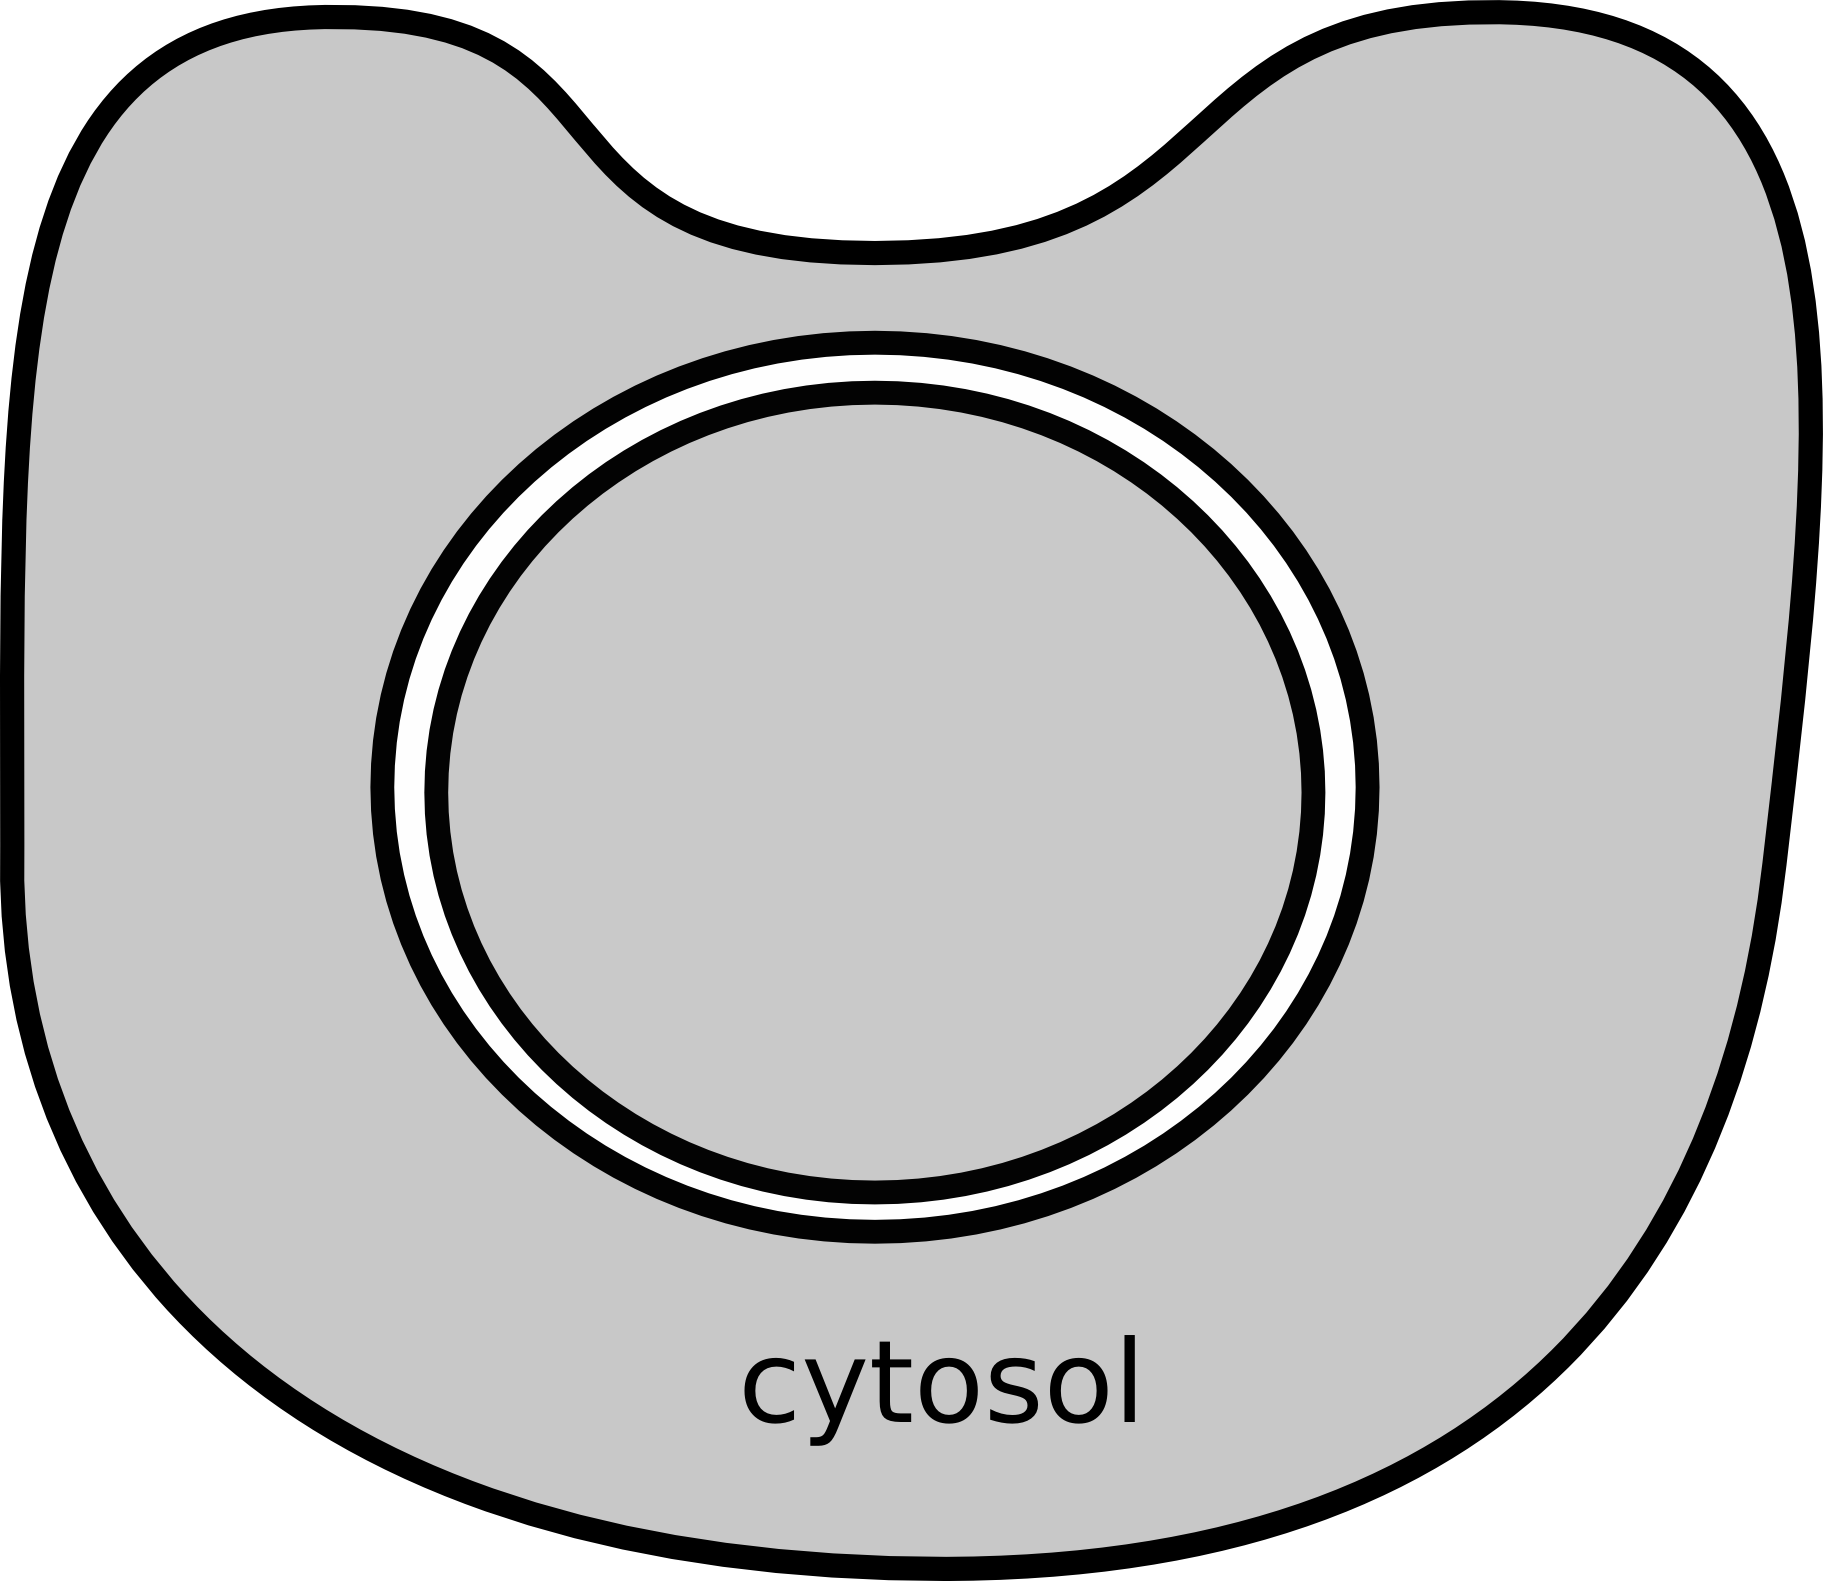
\includegraphics[scale = 0.4]{examples/compartment-cell.png}
% 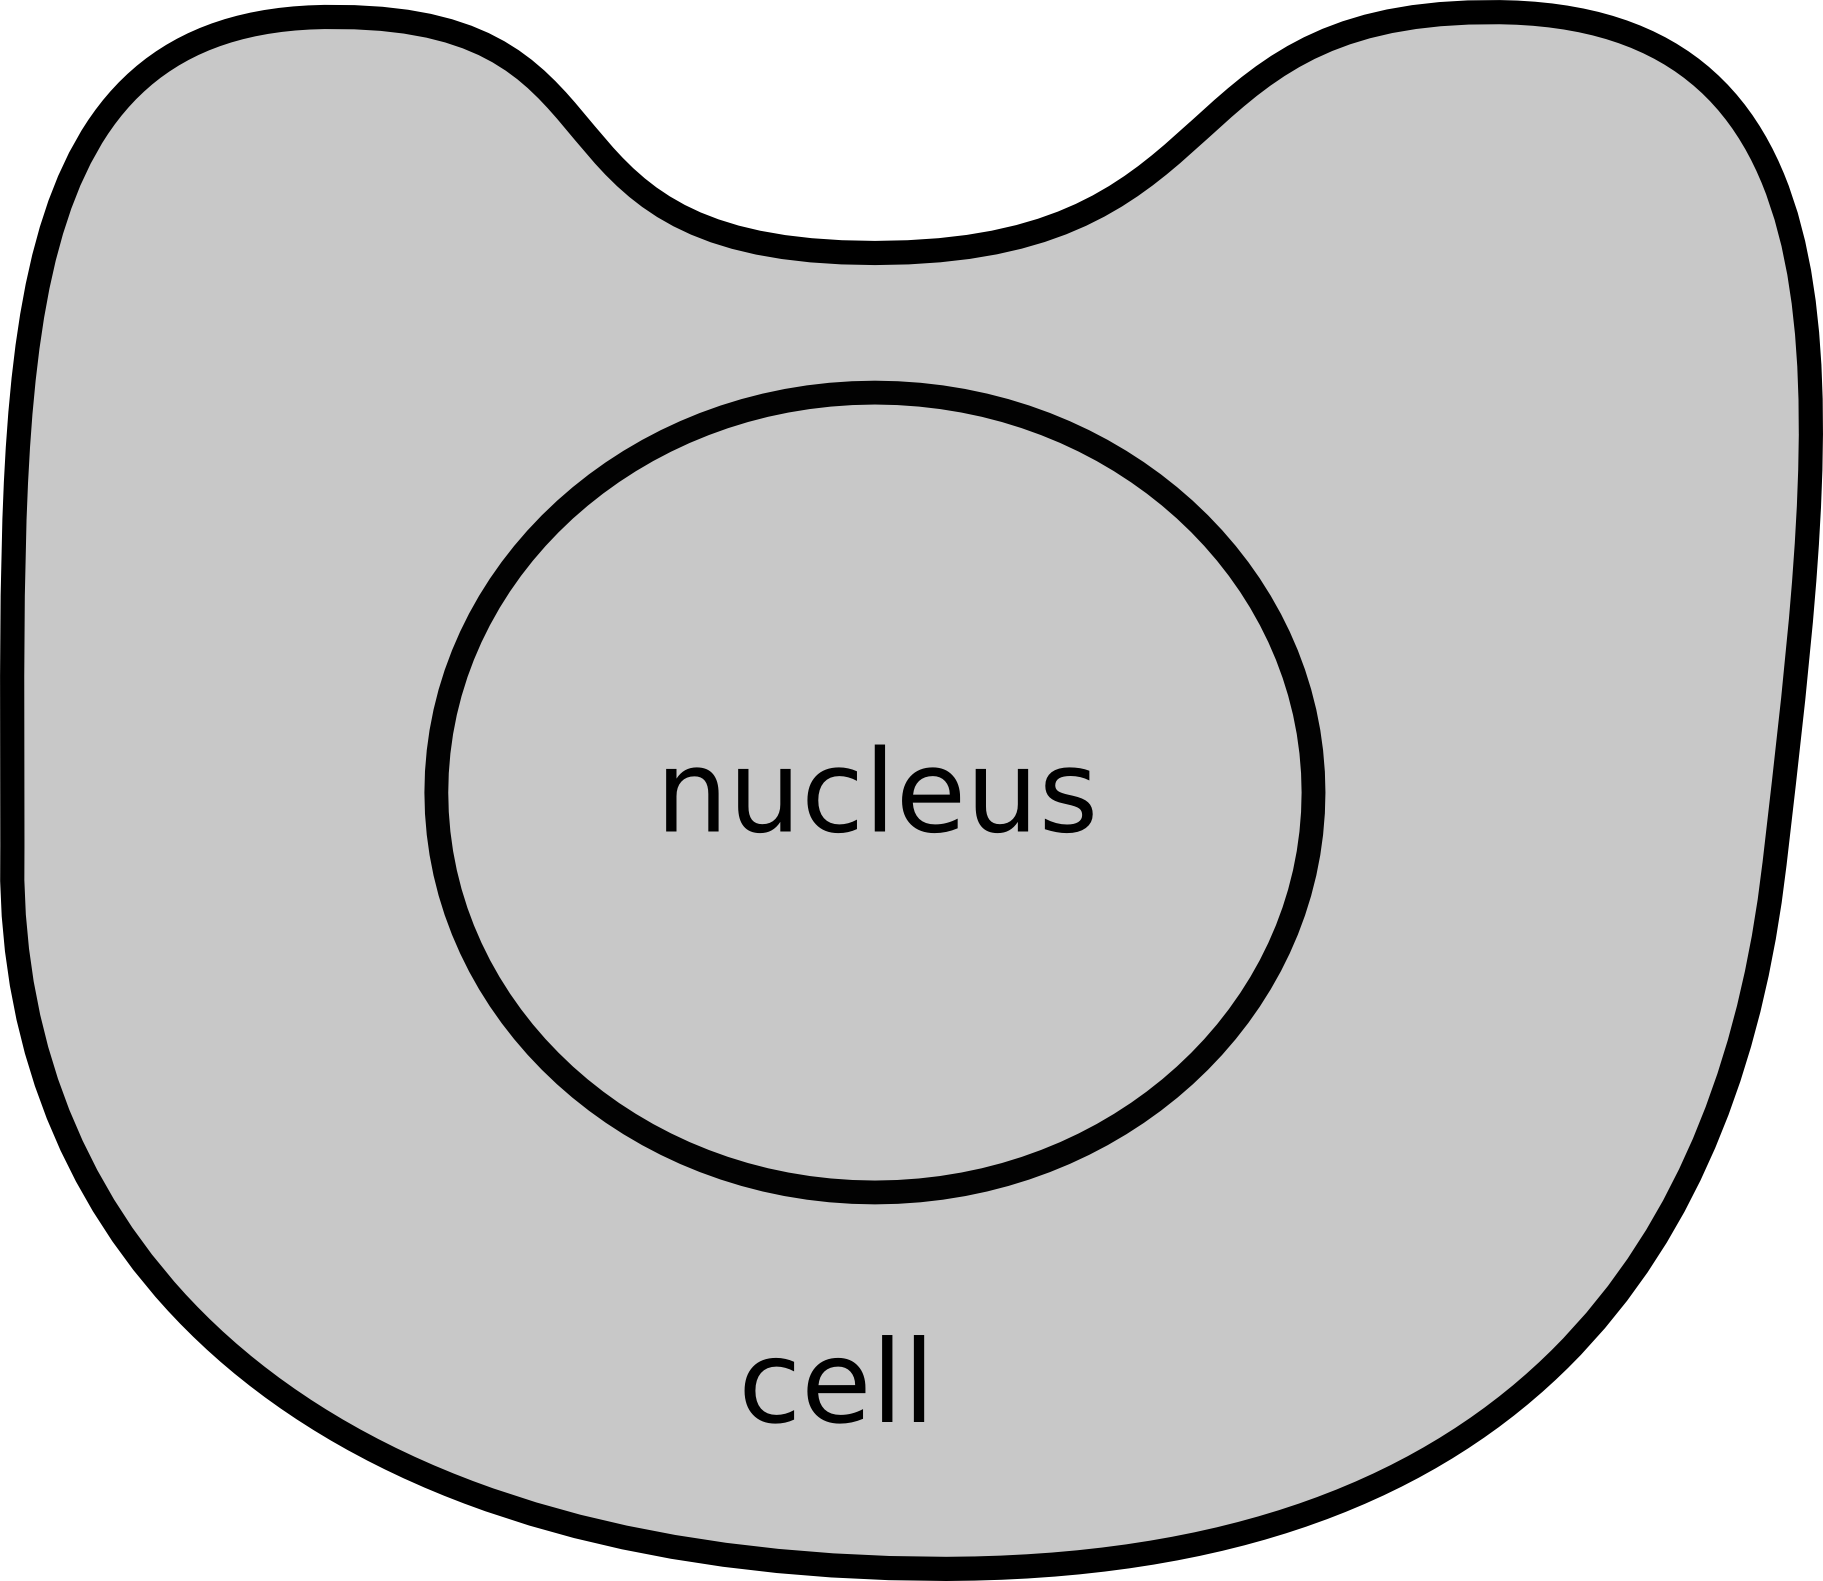
\includegraphics[scale = 0.4]{examples/compartment-cell-wrong.png}
 % \caption{Compartments can surround other compartments; in that case, both of the compartment's borders must still be shown, with the result that the separation is drawn as two lines. The example on the left is correct representation of the ``cytoplasm'' and the ``nucleus'', while the example on the right side shows an incorrect representation. }
%  \label{fig:two-comp}
%\end{figure}

%The example diagram in \fig{three-comp} represents three adjacent compartments.  Two of the compartments carry units of information.  Notice that these units of information do not overlap multiple membrane boundaries.

%\begin{figure}[H]
%  \centering
%  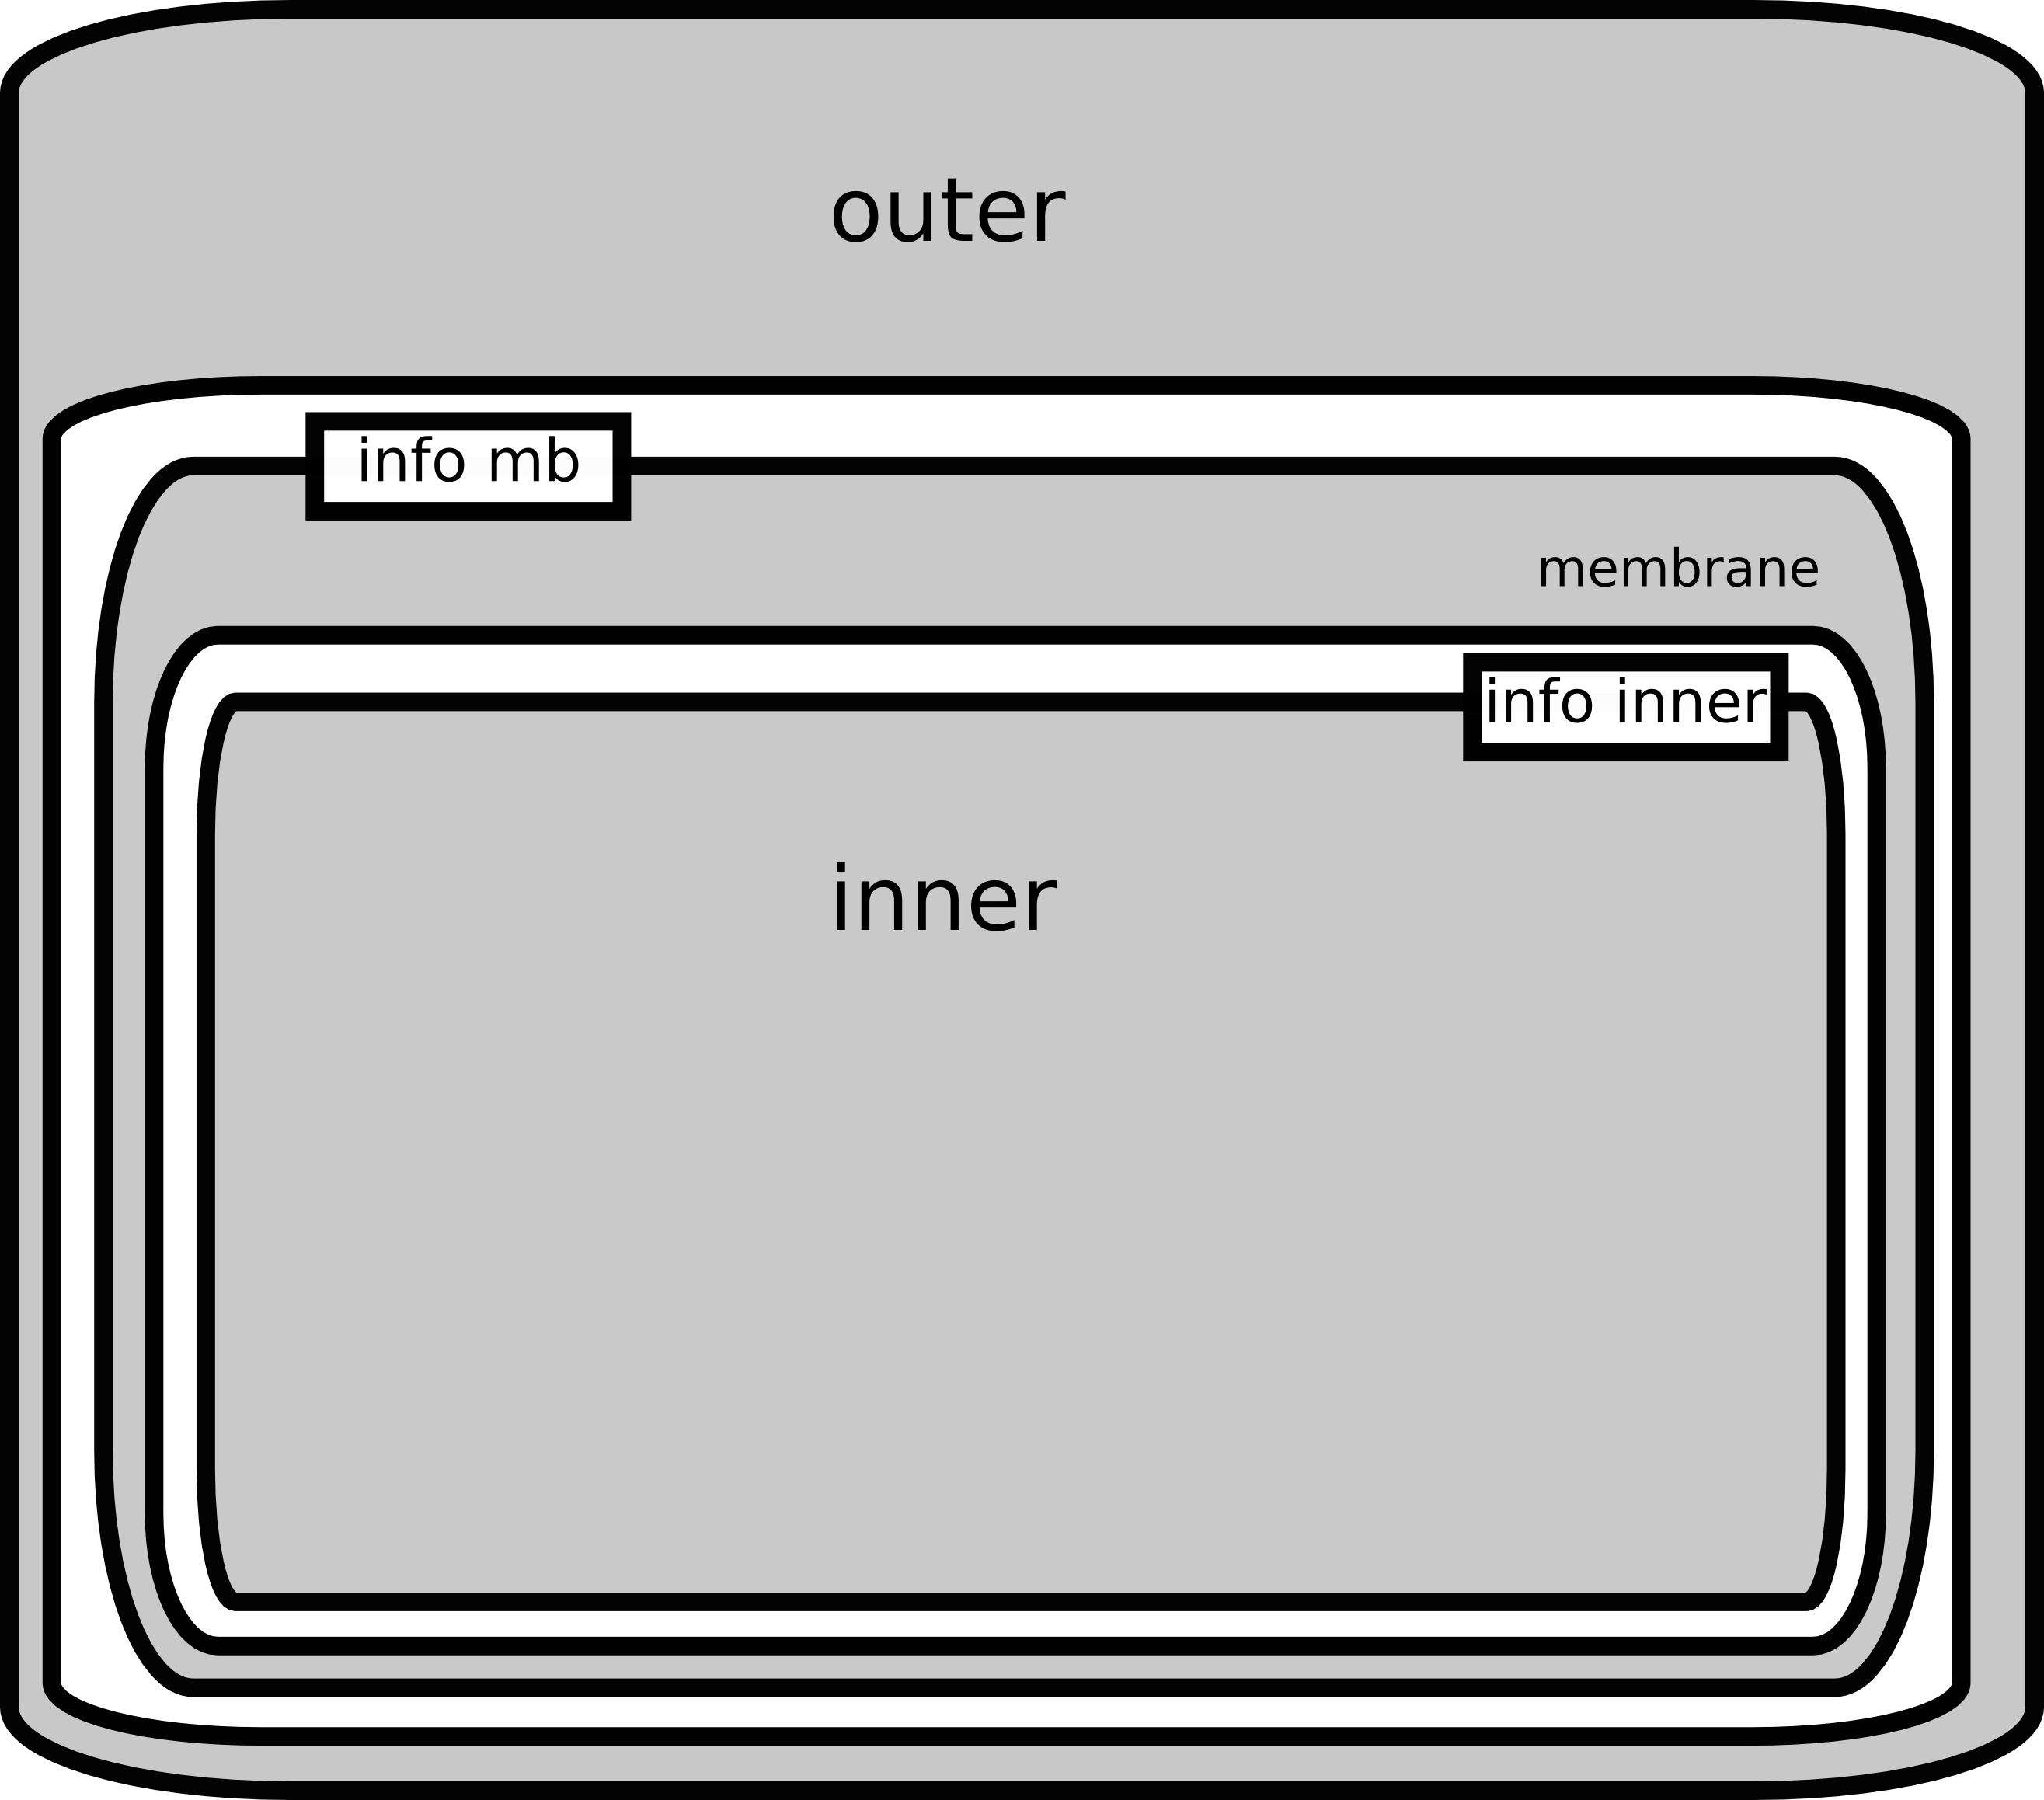
\includegraphics[scale = 0.4]{examples/compartment-3comp.png}
 % \caption{Illustration of units of information and surrounding compartments.}
 % \label{fig:three-comp}
%\end{figure}

It is important to note that a compartment never contains another compartment. To allow more aesthetically pleasing and understandable diagrams, compartments are allowed to overlap each other visually, but it must be kept in mind that this does not mean one compartment contains part or entire of the other compartment.  \fig{overlap} shows three semantically equivalent placement of compartments:

\begin{figure}[H]
  \centering
  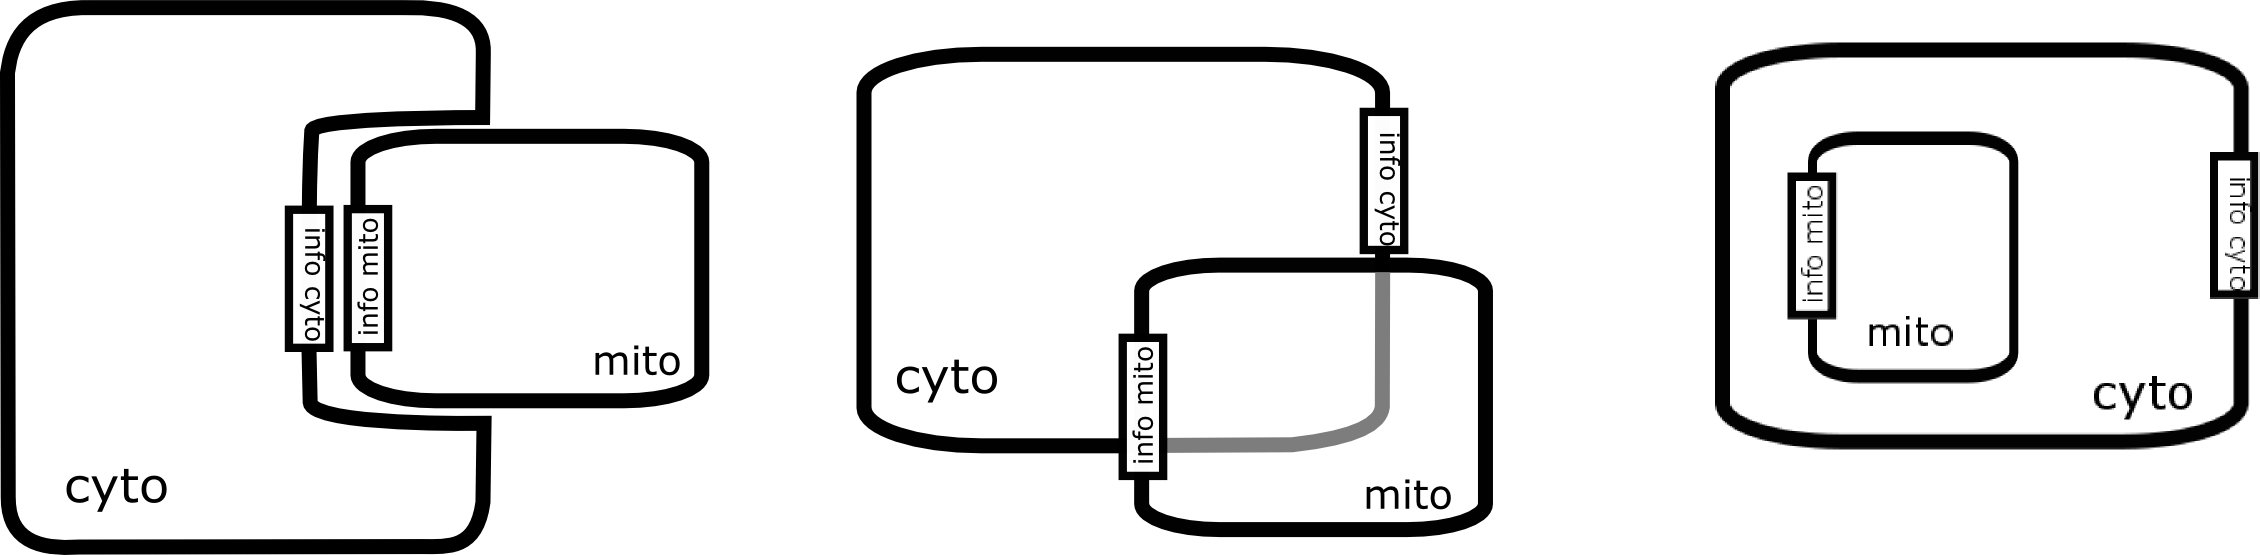
\includegraphics[scale = 0.4]{examples/compartment_overlapping.png}
  \caption{Overlapped compartments are permitted, but the overlap does not imply containment.}
  \label{fig:overlap}
\end{figure}

Overlapped (hidden) part of the compartment should not contain any object which could be covered by an overlapping compartment.  \fig{overlap-bad} illustrates the problem using an incorrect diagram.

\begin{figure}[H]
  \centering
  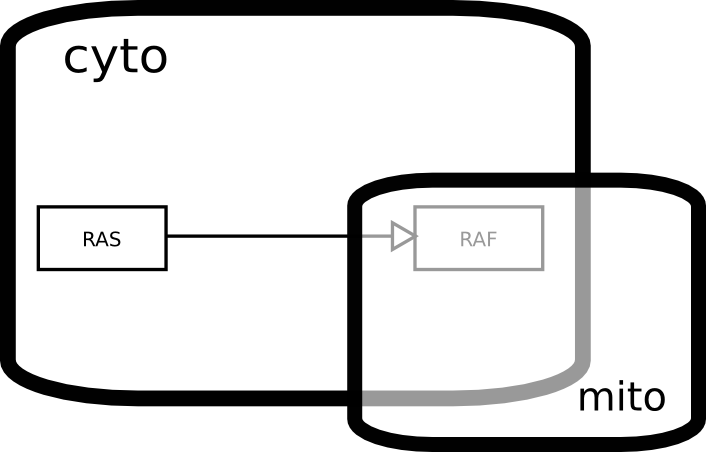
\includegraphics[scale = 0.45]{examples/compartment_overlapping_wrong.png}
  \caption{Example of an \textbf{incorrect} diagram.  Overlapped compartments must not obscure other objects.}
  \label{fig:overlap-bad}
\end{figure}

